\documentclass[11pt,fancychapters]{article}
\usepackage[a4paper, total={6in, 8in}]{geometry}
\usepackage{cite}
\usepackage{color}
\usepackage{xcolor}
\usepackage{empheq}
\usepackage{enumitem}
\usepackage{setspace}
\usepackage{hyperref}
\usepackage{minted}
\usepackage{acro}
\usepackage{amsmath}
\usepackage{amsthm}
\usepackage{amssymb}
\usepackage{multirow}
\usepackage{graphicx}
\usepackage{geometry}
\usepackage{subcaption}
\usepackage{cancel}
\usepackage[utf8]{inputenc}
\usepackage[english]{babel}
\usepackage{tcolorbox}
\usepackage{hyperref}
\usepackage{cleveref}
\usepackage{parskip}
\usepackage{tcolorbox}
\usepackage{float}
\usepackage{bm}
\usepackage{mathtools}
\usepackage{pgfplots}
 \geometry{
 a4paper,
 total={170mm,257mm},
 left=20mm,
 top=20mm,
 }
\pgfplotsset{width=8cm,compat=1.9}
\newcommand{\dbar}{{d\mkern-7mu\mathchar'26\mkern-2mu}}
\newcommand{\boxedeq}[2]{\begin{empheq}[box={\fboxsep=6pt\fbox}]{align}\label{#1}#2\end{empheq}}
\newcommand{\approptoinn}[2]{\mathrel{\vcenter{
  \offinterlineskip\halign{\hfil$##$\cr
    #1\propto\cr\noalign{\kern2pt}#1\sim\cr\noalign{\kern-2pt}}}}}
\newcommand{\appropto}{\mathpalette\approptoinn\relax}
\renewcommand*{\thesection}{\arabic{section}.}
\def\*#1{\mathbf{#1}}
\def\ab{ab}
\usepackage{tikz}
\usetikzlibrary{fit,calc,trees,positioning,arrows,chains,shapes.geometric,%
    decorations.pathreplacing,decorations.pathmorphing,shapes,%
    matrix,shapes.symbols,automata}
\geometry{top=1.3in,bottom=1.3in}

\DeclarePairedDelimiter\abs{\lvert}{\rvert}%
\DeclarePairedDelimiter\norm{\lVert}{\rVert}%

% Swap the definition of \abs* and \norm*, so that \abs
% and \norm resizes the size of the brackets, and the 
% starred version does not.
\makeatletter
\let\oldabs\abs
\def\abs{\@ifstar{\oldabs}{\oldabs*}}
%
\let\oldnorm\norm
\def\norm{\@ifstar{\oldnorm}{\oldnorm*}}
\makeatother

\begin{document}
\centerline{\huge{SUTD 2021 50.007 Final Examination}}

\begin{table}[ht]
\centering
\footnotesize
 \begin{tabular}{c c} 
James Raphael Tiovalen & 1004555
 \end{tabular}
\end{table}

\subsection*{Question 1 {\normalfont{[9 points]}}}

Consider the following 1D world with states a, b, c, d, and e where states a and e are exit states. There are 3 actions available: \textit{Left}, \textit{Right}, and \textit{Exit}. The \textit{Exit} action is only available in the exit states a and e where a reward of 100 and 10 can be obtained respectively. The transition probability $T(s, a, s') = P(s' | s, a) = 1$ such that each action is $100\%$ successful and the living reward/immediate reward $R(s, a, s') = 0$. Given this information, find the following:

\begin{table}[h!]
	\centering
	\begin{tabular}{| c | c | c | c | c |} 
		\hline
		$100$ & & & & $10$ \\
		\hline
		a & b & c & d & e \\
		\hline
	\end{tabular}
\end{table}

\begin{enumerate}[label=\textbf{(\arabic*)}]
	\item For $\gamma = 1$, what is the optimal policy? Answer by filling in the action that should be taken at each state in the table below. (Choose one from \{\textit{Left}, \textit{Right}, \textit{Exit}\}.)
	
	\begin{table}[h!]
		\centering
		\begin{tabular}{| c | c | c | c | c |} 
			\hline
			$100$ & \textit{Left} & \textit{Left} & \textit{Left} & $10$ \\
			\hline
			a & b & c & d & e \\
			\hline
		\end{tabular}
	\end{table}

	\item For $\gamma = 0.1$, what is the optimal policy? Answer by filling in the action that should be taken at each state in the table below. (Choose one from \{\textit{Left}, \textit{Right}, \textit{Exit}\}.)
	
	\begin{table}[h!]
		\centering
		\begin{tabular}{| c | c | c | c | c |} 
			\hline
			$100$ & \textit{Left} & \textit{Left} & \textit{Right} & $10$ \\
			\hline
			a & b & c & d & e \\
			\hline
		\end{tabular}
	\end{table}
\end{enumerate}

\subsection*{Question 2 {\normalfont{[12 points]}}}

Consider the following Bayesian network:

\begin{figure*}[h!]
	\centering
	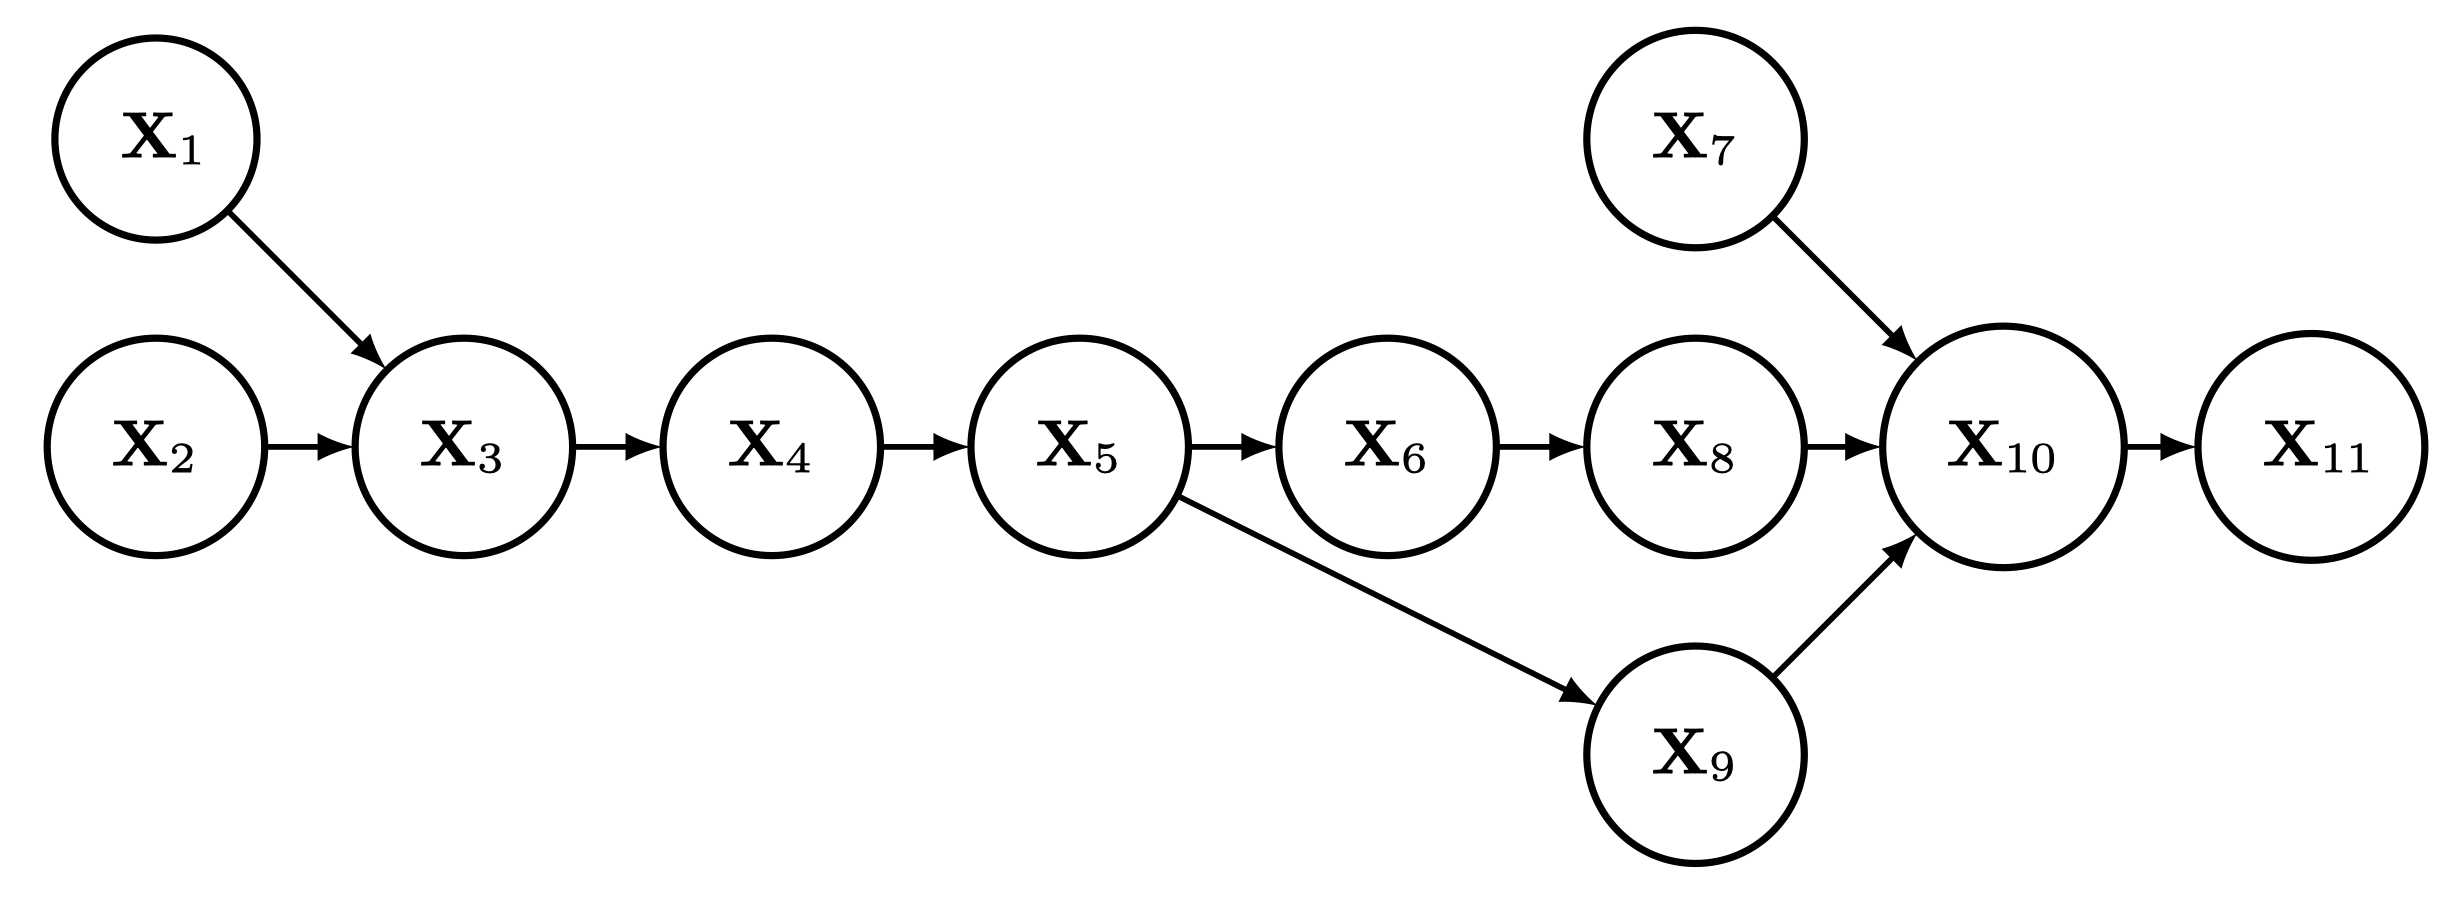
\includegraphics[scale=.17]{BN(a)1.png}
\end{figure*}

where the probability tables are as follows:

\begin{figure*}[h!]
	\centering
	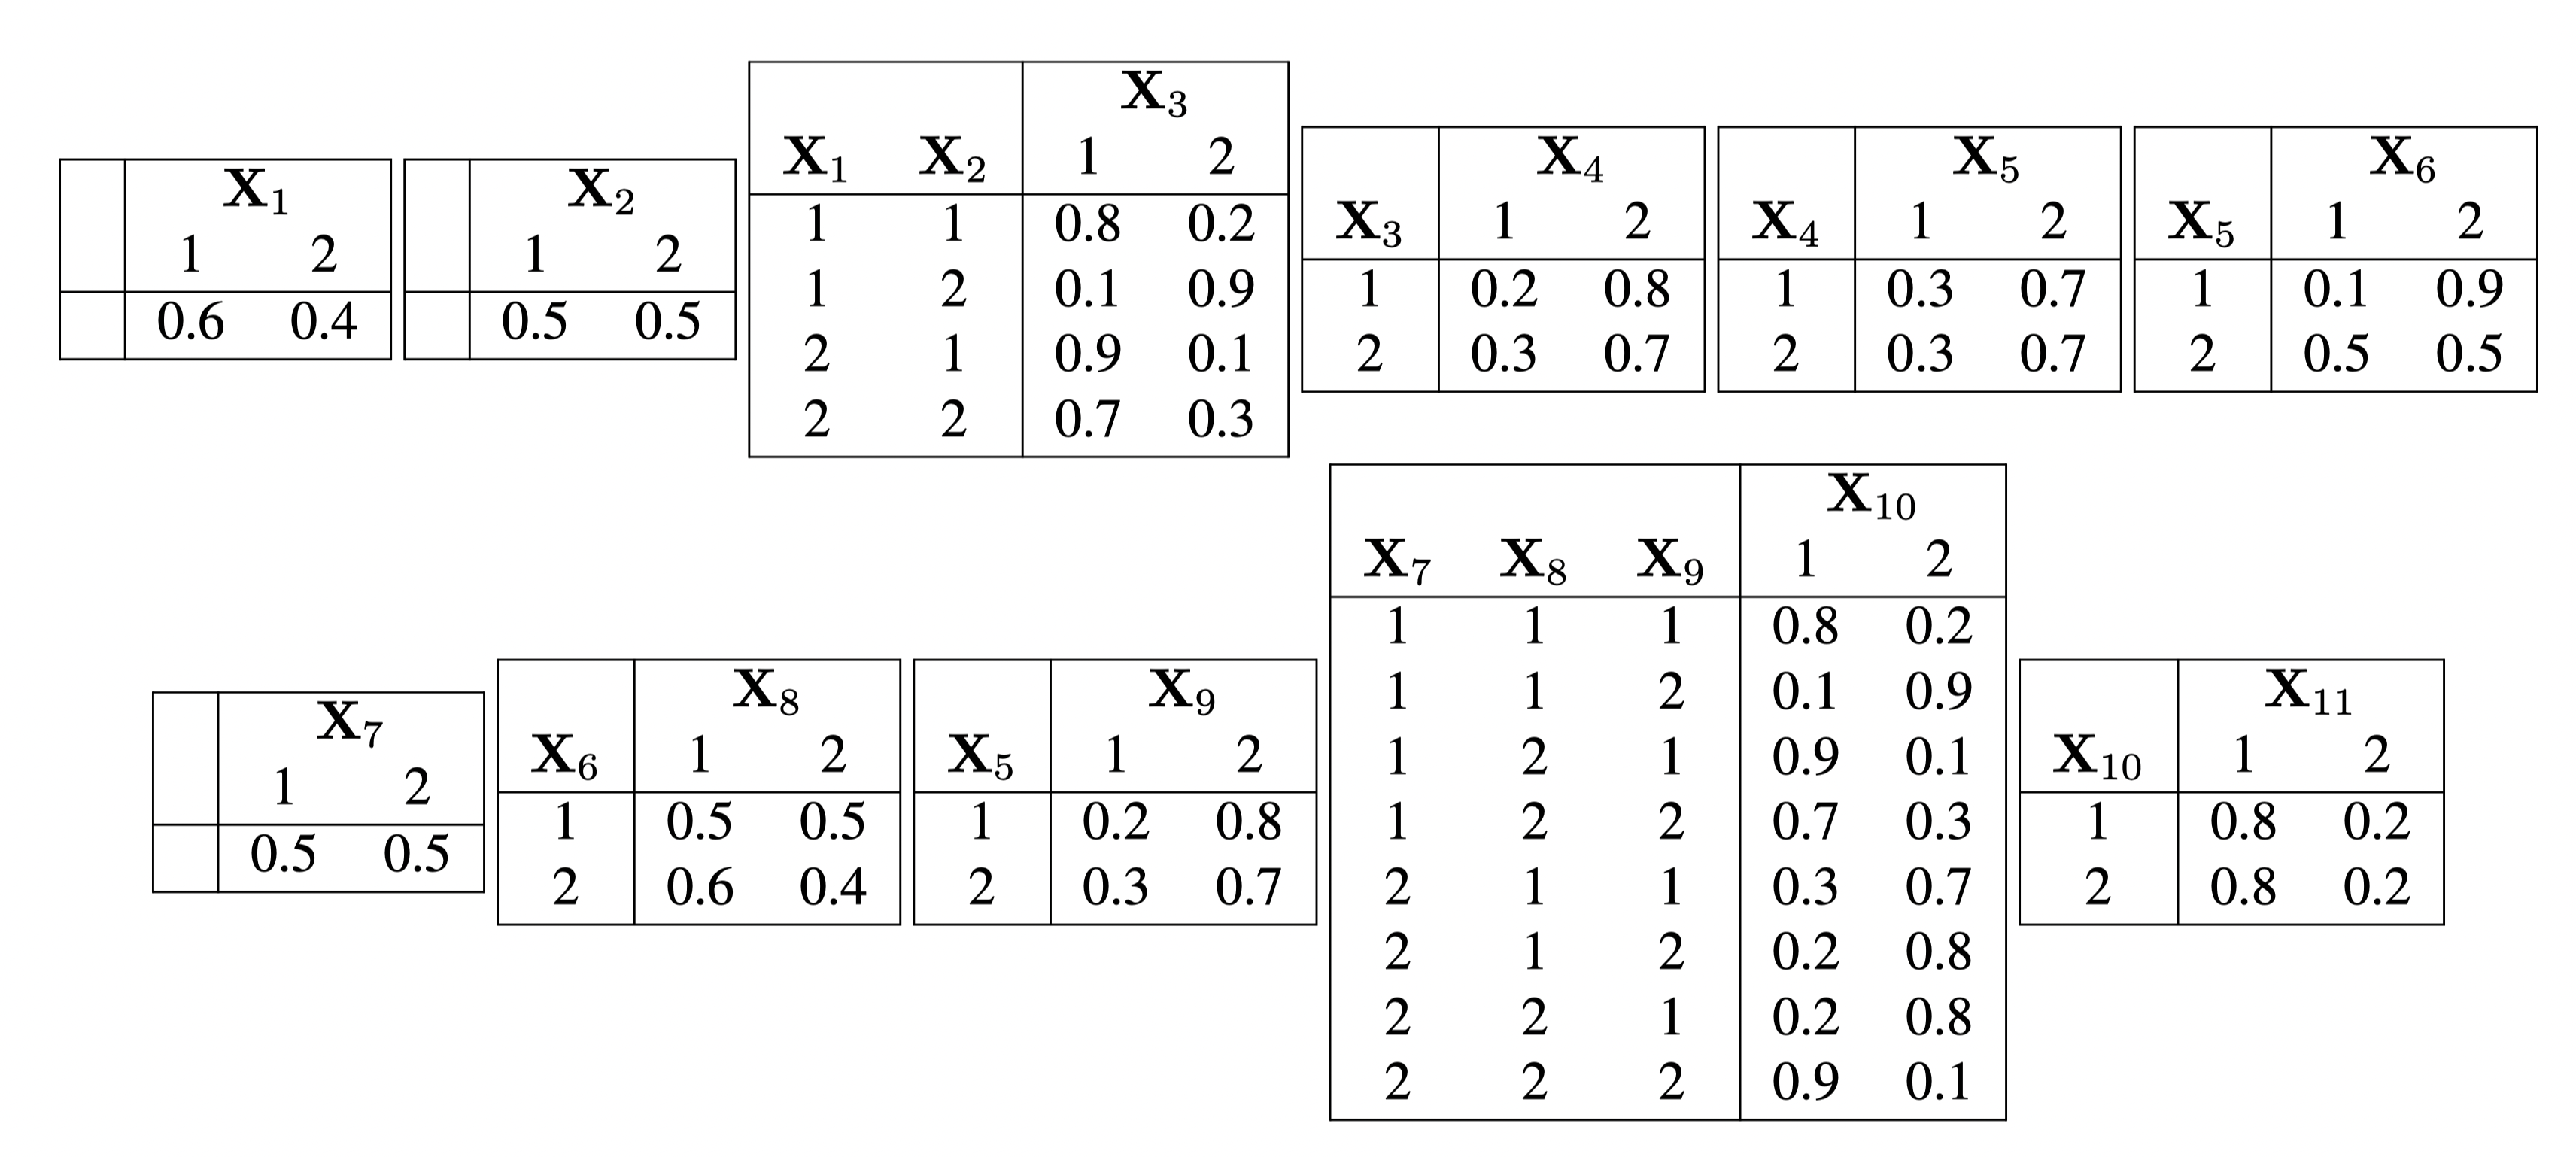
\includegraphics[scale=.13]{BN(b)11.png}
\end{figure*}

\pagebreak

\begin{enumerate}[label=\textbf{\alph*.}]
	\item Calculate $P(\textbf{X}_4 = 1) = 0.241$.
	\item Calculate $P(\textbf{X}_{10} = 1 | \textbf{X}_6 = 2, \textbf{X}_9 = 2, \textbf{X}_{11} = 1) = 0.41$.
\end{enumerate}

\subsection*{Question 3 {\normalfont{[1 point]}}}

A Generative Model learns the joint probability distribution $p(y | x)$, while a Discriminative Model learns the conditional probability distribution $p(x, y)$.

Answer: \textbf{False}.

\subsection*{Question 4 {\normalfont{[1 point]}}}

The Gaussian Mixture Model, or GMM for short, is a mixture model that uses a combination of normal or exponential probability distributions and requires the estimation of the mean and standard deviation parameters for each.

Answer: \textbf{False}.

\subsection*{Question 5 {\normalfont{[1 point]}}}

Many real-world problems have hidden variables (sometimes called latent variables), which are not observable in the data that are available for learning. The Expectation-Maximization algorithm can be used for searching for the appropriate model parameters in the presence of latent variables.

Answer: \textbf{True}.

\subsection*{Question 6 {\normalfont{[1 point]}}}

Logistic Regression is a discriminative classifier whereas Na\"{i}ve Bayes is a generative classifier.

Answer: \textbf{True}.

\subsection*{Question 7 {\normalfont{[12 points]}}}

Consider an MDP with 3 states: A, B, and C; and 2 actions: Clockwise and Counterclockwise. We do not know the transition function or the reward function for the MDP, but instead, we are given samples of what an agent actually experiences when it interacts with the environment (although, we do know that we do not remain the same state after taking an action). In this problem, instead of first estimating the transition and reward functions, we will directly estimate the $Q$ function using $Q$-learning. Assume, the discount factor, $\gamma$ is $0.5$ and the learning rate for $Q$-learning, $\alpha$ is $0.5$. Our current $Q$ function, $Q(s, a)$, is as follows:

\begin{table}[h!]
	\centering
	\begin{tabular}{| c | c | c | c |} 
		\hline
		& A & B & C \\
		\hline
		Clockwise & 1.501 & -0.451 & 2.730 \\
		\hline
		Counterclockwise & 3.153 & -7.055 & 2.133 \\
		\hline
	\end{tabular}
\end{table}

The agent encounters the following samples:

\begin{table}[h!]
	\centering
	\begin{tabular}{| c | c | c | c |} 
		\hline
		s & a & s' & r \\
		\hline
		A & Counterclockwise & C & 8.0 \\
		\hline
		C & Counterclockwise & A & 0.0 \\
		\hline
	\end{tabular}
\end{table}

Process the samples given above. Below fill in the $Q$-values (rounded off to 3 decimal points) after both samples have been accounted for sequentially.

\begin{enumerate}[label=\textbf{\arabic*.}]
	\item $Q(A, \text{clockwise}) = 1.501$
	\item $Q(A, \text{counterclockwise}) = 6.259$
	\item $Q(B, \text{clockwise}) = -0.451$
	\item $Q(B, \text{counterclockwise}) = -7.055$
	\item $Q(C, \text{clockwise}) = 2.730$
	\item $Q(C, \text{counterclockwise}) = 2.631$
\end{enumerate}

\subsection*{Question 8 {\normalfont{[5 points]}}}

Which of the following statements are correct?

\begin{enumerate}[label=\textbf{\alph*.}]
	\item The Viterbi algorithm is used for decoding. When doing decoding, we assume we know the exact values for both the transition and emission parameters.
	\item The Viterbi and the forward-backward algorithm discussed in class have different time complexity.
	\item We can use the hard EM or the soft EM algorithm to perform unsupervised learning of the HMM. The E-step of the hard EM algorithm will be less expensive than the soft EM algorithm in terms of time complexity.
	\item In a hidden Markov model that we learned in class, the very first variable that is generated is $y_0 = \text{START}$, whose Markov blanket only consists of one variable, which is $y_1$.
\end{enumerate}

Answer: \textbf{a} and \textbf{d}.

\subsection*{Question 9 {\normalfont{[5 points]}}}

Which of the following statements are correct?

\begin{enumerate}[label=\textbf{\alph*.}]
	\item Based on the Bayes' ball algorithm, if there exists a path from X to Z that is open, we say the two variables X and Z are independent. Otherwise, they are dependent.
	\item When learning Bayesian network structures from data, we should not use the log-likelihood as the criteria for selecting the structure of a Bayesian network. If we do so, we might find that in general, a more complex structure is always preferred over a simpler structure as a more complex structure tends to fit the data better.
	\item The hidden Markov model can not be viewed as a Bayesian network.
	\item The naive Bayes model can be regarded as a special Bayesian network.
\end{enumerate}

Answer: \textbf{b} and \textbf{d}.

\subsection*{Question 10 {\normalfont{[12 points]}}}

Consider the following Bayesian network. All nodes can take 4 different values: \{1, 2, 3, 4\}.

\begin{figure*}[h!]
	\centering
	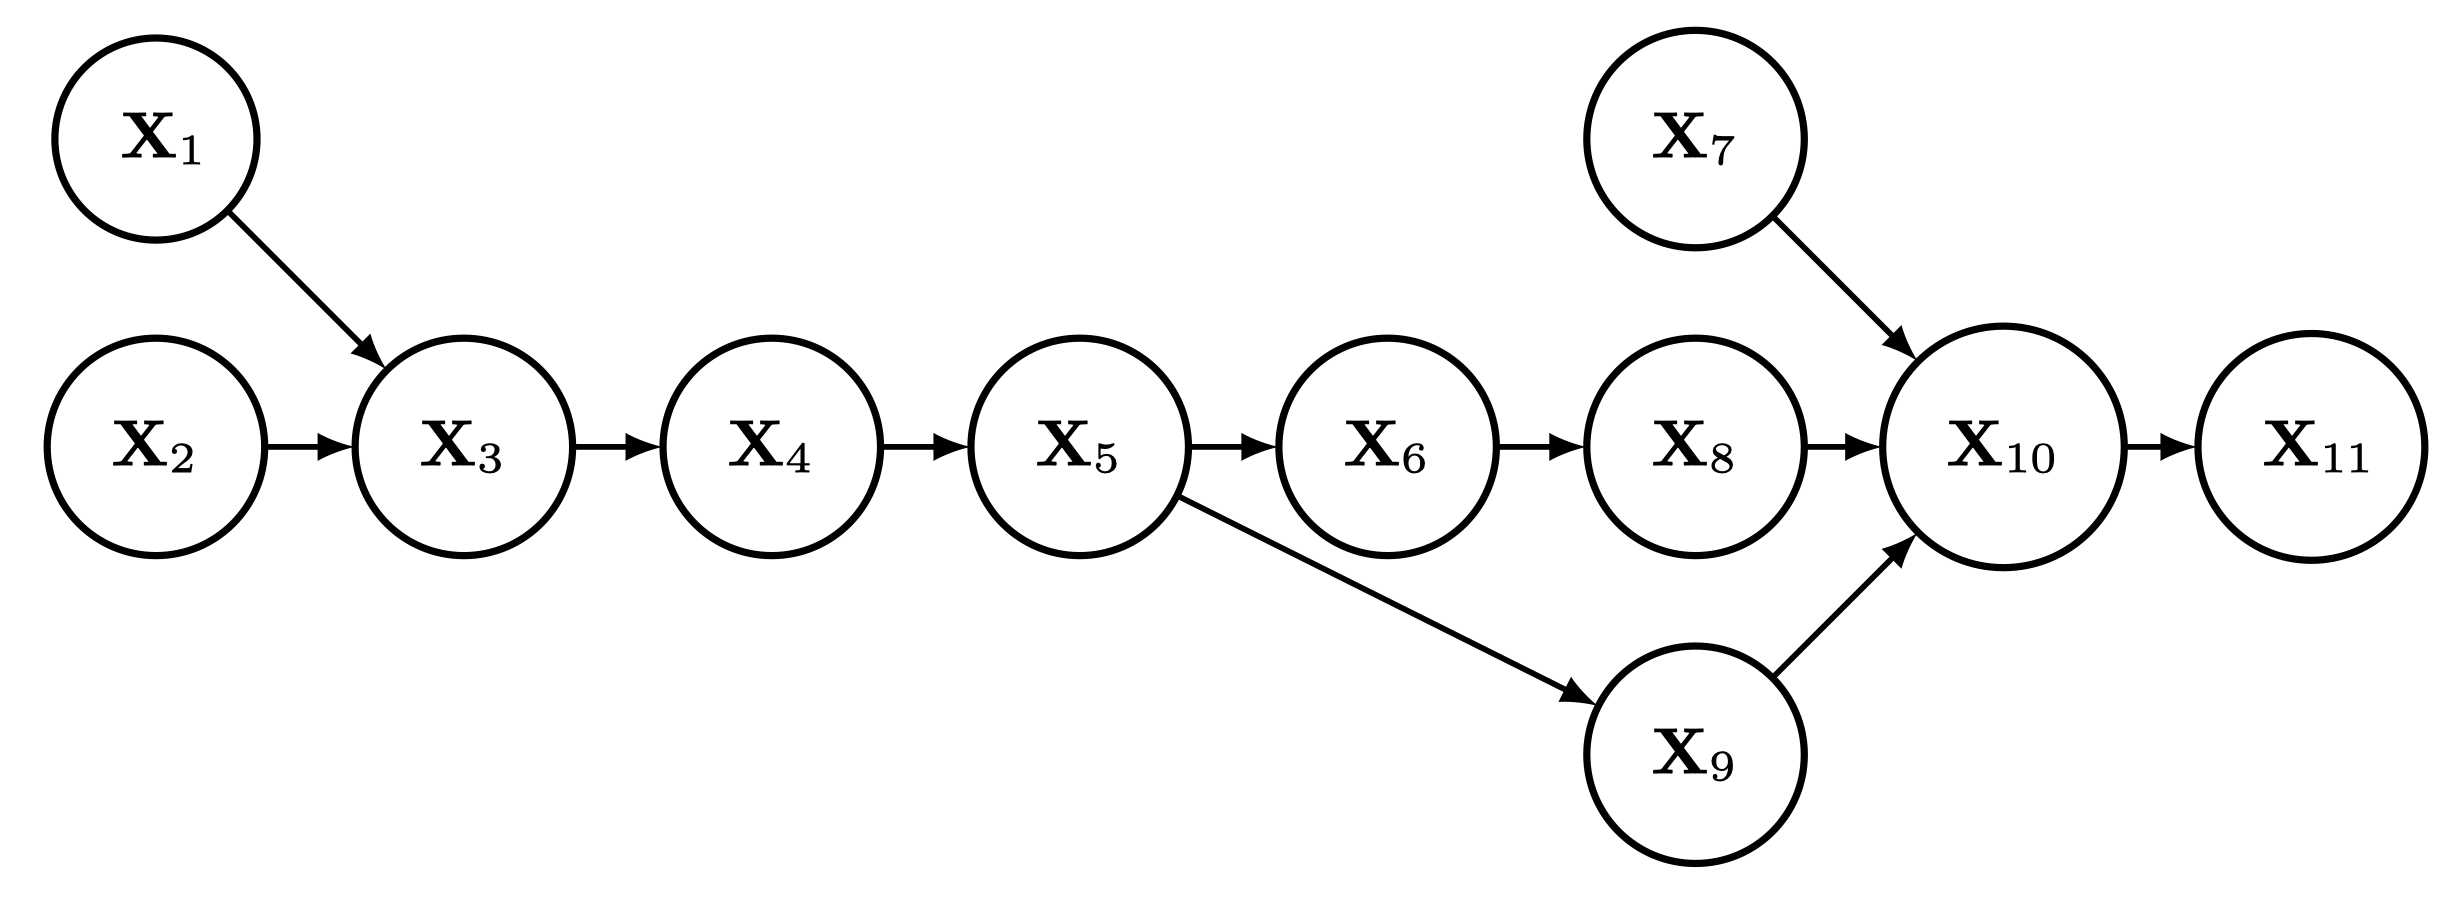
\includegraphics[scale=.17]{BN(a)1.png}
\end{figure*}

\begin{enumerate}[label=\textbf{\alph*.}]
	\item What is the number of free parameters for this Bayesian network? Answer (integer): 321.
	\item Without knowing the actual value of any node, are nodes $\textbf{X}_1$ and $\textbf{X}_7$ independent of each other? Answer (yes/no): yes.
	\item If we know the value of nodes $\textbf{X}_6$ and $\textbf{X}_{10}$, are nodes $\textbf{X}_1$ and $\textbf{X}_7$ independent of each other? Answer (yes/no): no.
	\item Is $P(\textbf{X}_3 | \textbf{X}_4) = P(\textbf{X}_3 | \textbf{X}_6, \textbf{X}_4)$ always true no matter what values $\textbf{X}_3$, $\textbf{X}_4$, and $\textbf{X}_6$ take? Answer (yes/no): yes.
\end{enumerate}

\subsection*{Question 11 {\normalfont{[1 point]}}}

The soft-EM algorithm comes with a guarantee: it will always converge to a global optimum of the objective function, no matter how you do the initialization.

Answer: \textbf{False}.

\subsection*{Question 12 {\normalfont{[1 point]}}}

One task that we can perform with a hidden Markov model (HMM) is to predict the underlying part-of-speech sequence for each input sentence. Under this setting, we can say that the HMM can help us find a mapping between two structured spaces: the input space consists of all possible sentences and the output space consists of all possible part-of-speech tag sequences.

Answer: \textbf{True}.

\subsection*{Question 13 {\normalfont{[1 point]}}}

The EM algorithm can be used for unsupervised learning of a hidden Markov model.

Answer: \textbf{True}.

\subsection*{Question 14 {\normalfont{[1 point]}}}

The forward-backward algorithm involves two procedures that perform the calculation of the forward scores and the backward scores respectively. In practice, as these two procedures do not depend on each other, one can choose to calculate the backward scores first and then the forward scores.

Answer: \textbf{True}.

\subsection*{Question 15 {\normalfont{[1 point]}}}

The space complexity of the forward-backward algorithm is $O(nT)$ for each instance, where $n$ is the length of the input sequence, and $T$ is the number of possible output states at each position.

Answer: \textbf{True}.

\subsection*{Question 16 {\normalfont{[1 point]}}}

Hidden Markov models can be regarded as a special class of Bayesian networks.

Answer: \textbf{True}.

\subsection*{Question 17 {\normalfont{[12 points]}}}

Consider a HMM where the transition and emission probabilities are given as follows:

\begin{table}[h!]
	\centering
	\begin{tabular}{| c | c | c | c | c |}
		\hline
		$a_{u, v} ~ | ~ u \backslash v$ & X & Y & Z & STOP \\
		\hline
		START & 0.2 & 0.4 & 0.4 & 0 \\
		\hline
		X & 0.2 & 0.2 & 0.2 & 0.4 \\
		\hline
		Y & 0.2 & 0.2 & 0.2 & 0.4 \\
		\hline
		Z & 0.4 & 0.2 & 0.2 & 0.2 \\ 
		\hline
	\end{tabular}
\end{table}

\begin{table}[h!]
	\centering
	\begin{tabular}{| c | c | c | c |}
		\hline
		$b_u(o) ~ | ~ u \backslash o$ & $\textbf{a}$ & $\textbf{b}$ & $\textbf{c}$ \\
		\hline
		X & 0.6 & 0.1 & 0.3 \\
		\hline
		Y & 0.4 & 0.1 & 0.5 \\
		\hline
		Z & 0.5 & 0.4 & 0.1 \\
		\hline
	\end{tabular}
\end{table}

We can use the forward-backward algorithm to calculate the joint probability distribution $P(y_2, x_1 = \textbf{a}, x_2 = \textbf{b}, x_3 = \textbf{a})$ where $\textbf{x} = (x_1, x_2, x_3)$ is the observation sequence and $\textbf{y} = (y_1, y_2, y_3)$ is the tag sequence.

\begin{enumerate}[label=\textbf{\arabic*.}]
	\item Calculate the backward score $P(x_2 = \textbf{b}, x_3 = \textbf{a} | y_2 = Y) = 0.01$.
	\item Calculate $P(y_2 = Y, x_1 = \textbf{a}, x_2 = \textbf{b}, x_3 = \textbf{a}) = 0.00096$.
\end{enumerate}

\subsection*{Question 18 {\normalfont{[10 points]}}}

Assume that we have the following training set available for us to estimate the model parameters under the maximum likelihood estimation (MLE):

\begin{table}[h!]
	\centering
	\begin{tabular}{| c | c |}
		\hline
		State sequence & Observation sequence \\
		\hline
		(X, Y, Z) & (\textbf{a}, \textbf{c}, \textbf{a}) \\
		\hline
		(X, Z, Y) & (\textbf{a}, \textbf{b}, \textbf{a}) \\
		\hline
		(Z, Y, X, Z) & (\textbf{b}, \textbf{c}, \textbf{a}, \textbf{b}) \\
		\hline
		(Z, X, Y) & (\textbf{c}, \textbf{b}, \textbf{a}) \\
		\hline
		(X, Y) & (\textbf{a}, \textbf{b}) \\
		\hline
	\end{tabular}
\end{table}

Fill up the following transition and emission probability tables. (Round all the numbers to 3 decimal places.)

\begin{table}[h!]
	\centering
	\begin{tabular}{| c | c | c | c | c |}
		\hline
		$a_{u, v} ~ | ~ u \backslash v$ & X & Y & Z & STOP \\
		\hline
		START & 0.6 & 0 & 0.4 & 0 \\
		\hline
		X & 0 & 0.6 & 0.4 & 0 \\
		\hline
		Y & 0.2 & 0 & 0.2 & 0.6 \\
		\hline
		Z & 0.2 & 0.4 & 0 & 0.4 \\ 
		\hline
	\end{tabular}
\end{table}

\begin{table}[h!]
	\centering
	\begin{tabular}{| c | c | c | c |}
		\hline
		$b_u(o) ~ | ~ u \backslash o$ & $\textbf{a}$ & $\textbf{b}$ & $\textbf{c}$ \\
		\hline
		X & 0.8 & 0.2 & 0 \\
		\hline
		Y & 0.4 & 0.2 & 0.4 \\
		\hline
		Z & 0.2 & 0.6 & 0.2 \\
		\hline
	\end{tabular}
\end{table}

\subsection*{Question 19 {\normalfont{[13 points]}}}

Consider a HMM where the transition and emission probabilities are given as follows. Use the Viterbi algorithm discussed in class to find the optimal state sequence for a given input observation sequence (\textbf{a}, \textbf{c}, \textbf{b}).

\begin{table}[h!]
	\centering
	\begin{tabular}{| c | c | c | c | c |}
		\hline
		$a_{u, v} ~ | ~ u \backslash v$ & X & Y & Z & STOP \\
		\hline
		START & 0.2 & 0.4 & 0.4 & 0 \\
		\hline
		X & 0.2 & 0.2 & 0.1 & 0.5 \\
		\hline
		Y & 0.1 & 0.1 & 0.1 & 0.7 \\
		\hline
		Z & 0.2 & 0.5 & 0.1 & 0.2 \\ 
		\hline
	\end{tabular}
\end{table}

\begin{table}[h!]
	\centering
	\begin{tabular}{| c | c | c | c |}
		\hline
		$b_u(o) ~ | ~ u \backslash o$ & $\textbf{a}$ & $\textbf{b}$ & $\textbf{c}$ \\
		\hline
		X & 0.6 & 0.1 & 0.3 \\
		\hline
		Y & 0.3 & 0.1 & 0.6 \\
		\hline
		Z & 0.5 & 0.4 & 0.1 \\
		\hline
	\end{tabular}
\end{table}

Fill up the blanks in the steps that lead to the final answer.

\textbf{Base case:}

\begin{equation*}
	\pi(0, \text{START}) = 1
\end{equation*}

\textbf{Moving forward:}

\begin{itemize}
	\item[] $k = 1$
	\begin{align*}
		\pi(1, X) &= 0.12 \\
		\pi(1, Y) &= 0.12 \\
		\pi(1, Z) &= 0.2
	\end{align*}
	
	\item[] $k = 2$
	\begin{align*}
		\pi(2, X) &= 0.012 \\
		\pi(2, Y) &= 0.06 \\
		\pi(2, Z) &= 0.002
	\end{align*}

	\item[] $k = 3$
	\begin{align*}
		\pi(3, X) &= 0.0006 \\
		\pi(3, Y) &= 0.0006 \\
		\pi(3, Z) &= 0.0024
	\end{align*}
	
	\item[] $k = 4$
	\begin{align*}
		\pi(4, \text{STOP}) &= 0.00048
	\end{align*}
\end{itemize}

\textbf{Backtracking:}

\begin{align*}
	y_3^* &= Z ~ \text{(Choose one from the set \{X, Y, Z\})} \\
	y_2^* &= Y ~ \text{(Choose one from the set \{X, Y, Z\})} \\
	y_1^* &= Z ~ \text{(Choose one from the set \{X, Y, Z\})}
\end{align*}

\end{document}
